\documentclass[12pt,a4paper]{article}

% --------------------
% Paquetes necesarios
% --------------------
\usepackage[spanish]{babel}     % Idioma español
\usepackage[utf8]{inputenc}     % Codificación UTF-8
\usepackage[T1]{fontenc}        % Codificación de fuente
\usepackage{fancyhdr}           % Para personalizar encabezados y pies
\usepackage{hyperref}           % Para hipervínculos en el índice
\usepackage{lipsum}             % Para generar texto de ejemplo
\usepackage{graphicx}           % Para insertar imágenes

% --------------------
% Información del trabajo
% --------------------
\newcommand{\miNombre}{Pedro González Fernández}
\newcommand{\miAsignatura}{Sistemas de Big Data}
\newcommand{\tituloTrabajo}{Análisis de Gráficos bajo la GESTALT}

% --------------------
% Configuración de encabezado/pie
% --------------------
\pagestyle{fancy}
\fancyhf{} % limpiar encabezados y pies
\fancyhead[L]{\miNombre}       % Cabecero izquierdo
\fancyhead[R]{\miAsignatura}   % Cabecero derecho

\fancyfoot[C]{\thepage}        % Pie centro: número de página

% --------------------
% Título del documento
% --------------------
\title{\tituloTrabajo \\ \large}
\author{\miNombre}
\date{\today}

% --------------------
% Documento
% --------------------
\begin{document}

\maketitle             % Genera título
\begin{figure}[h]
    \centering
    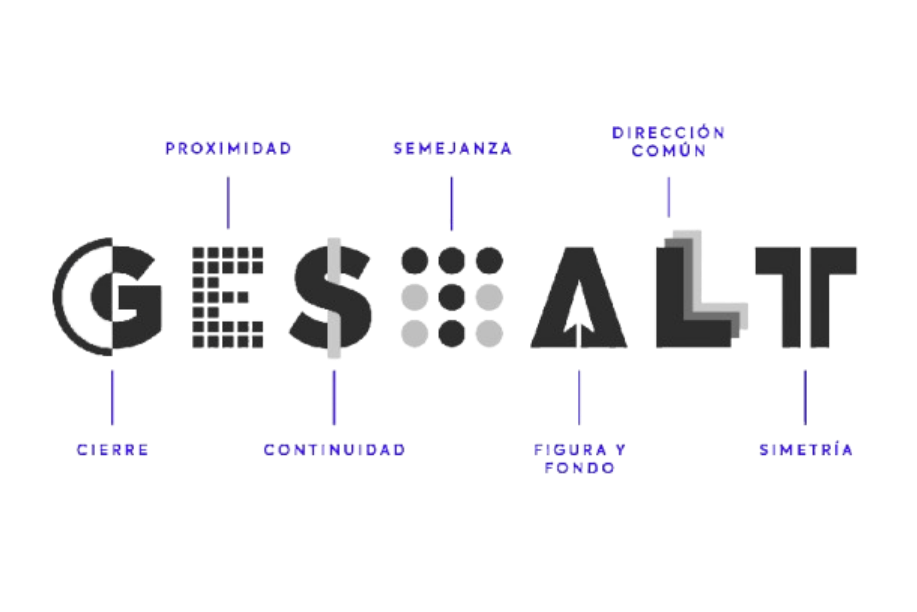
\includegraphics[width=0.7\textwidth]{gestalt.png}
    \label{fig:portada}
\end{figure}
\tableofcontents       % Genera índice
\newpage               % Nueva página después del índice

% --------------------
% Secciones
% --------------------
\section{Enunciado}
En este trabajo se presentan tres representaciones gráficas que serán analizadas a partir de los principios de la Gestalt. Se evaluará de qué manera dichos principios \textbf{influyen en la percepción visual} y se propondrán posibles mejoras orientadas a \textbf{optimizar la claridad} y la \textbf{efectividad comunicativa} de cada gráfico.

\section{Desarrollo}
\subsection{Casos de COVID en Singapur}
\begin{figure}[h]
    \centering
    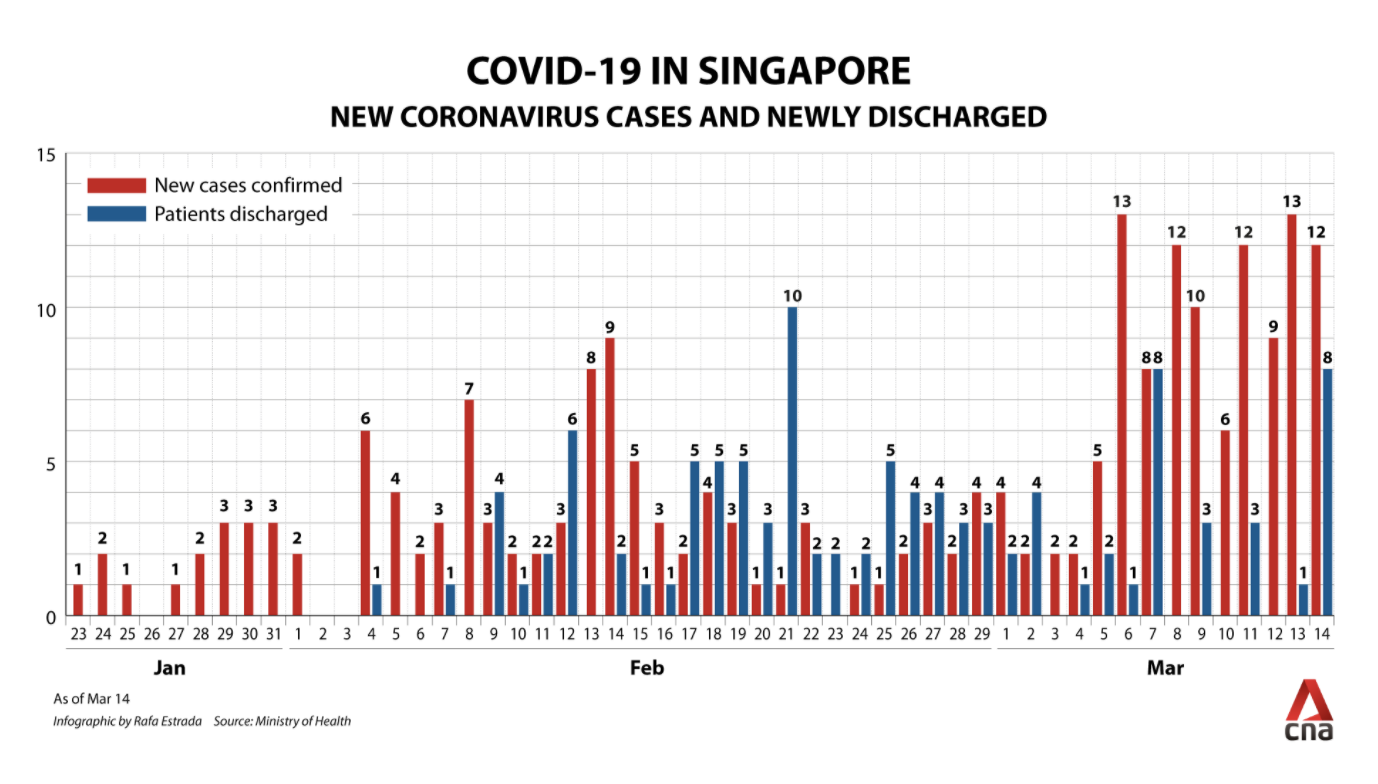
\includegraphics[width=0.7\textwidth]{graf1.png}
    \caption{Gráfico sobre casos de COVID en Singapur.}
    \label{fig:graf1}
\end{figure}
\subsubsection{Análisis}

\paragraph{Proximidad:}
Las barras de 'New cases' y 'Patients discharged' se presentan \textbf{agrupadas por meses}. La distancia mayor entre los \textbf{grupos mensuales} respecto a la existente entre barras de un mismo mes permite que el cerebro las perciba como \textbf{unidades diferenciadas}, facilitando así la \textbf{comparación temporal}.

\paragraph{Semejanza:} 
El uso de \textbf{colores distintos} posibilita identificar con claridad las \textbf{variables representadas}. Esto favorece la \textbf{agrupación visual} de las barras del mismo color a lo largo del gráfico.

\paragraph{Figura - Fondo:}
Las barras se constituyen en la \textbf{figura principal} y \textbf{destacan de manera nítida sobre el fondo}, que incluye una \textbf{cuadrícula sutil} a modo de soporte sin distraer la atención. Esto refuerza una \textbf{jerarquía visual clara}.

\paragraph{Simetría y orden:}
La disposición es \textbf{equilibrada y coherente}: los ejes están alineados, las etiquetas se presentan de forma consistente y el espacio se distribuye uniformemente. Todo ello contribuye a una \textbf{lectura profesional y comprensible}.

\subsubsection{Mejoras}

\paragraph{Continuidad:}
La secuencia temporal de izquierda a derecha sugiere \textbf{continuidad}; sin embargo, esta podría reforzarse mediante un \textbf{gráfico de líneas}. Este tipo de representación facilitaría una \textbf{percepción más fluida y continua de los datos}, mientras que el formato de barras puede interrumpir parcialmente dicha sensación.

\paragraph{Conectividad:}
Las barras, al ser elementos independientes, no permiten una \textbf{conexión directa} entre datos. Un gráfico de líneas solventaría esta limitación al \textbf{enlazar los puntos} y \textbf{reforzar la conectividad}. No obstante, en este caso la \textbf{proximidad} y la \textbf{semejanza} resultan suficientes para transmitir la información con claridad.

\newpage

\subsection{Jóvenes frente a 'Boomers'}
\begin{figure}[h]
    \centering
    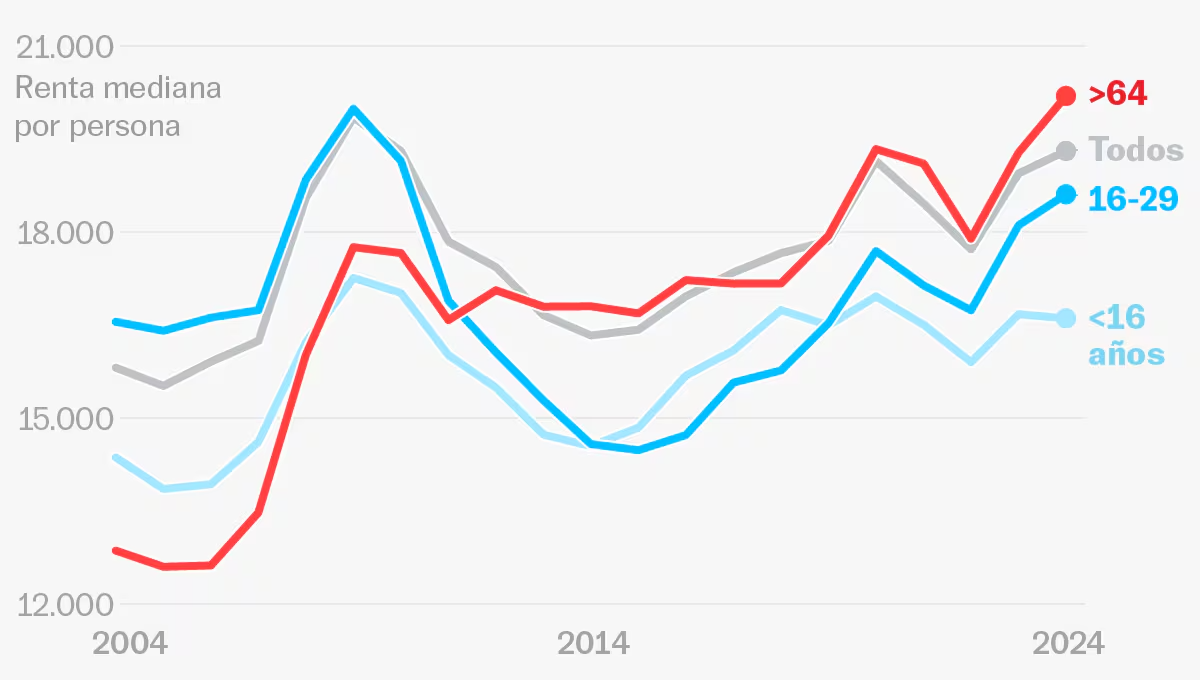
\includegraphics[width=0.7\textwidth]{graf2.png}
    \caption{Gráfico comparativo entre jóvenes y 'boomers' en aspectos económicos y sociales.}
    \label{fig:graf2}
\end{figure}
\subsubsection{Análisis}

\paragraph{Semejanza:}
Cada \textbf{línea} se representa con un \textbf{color diferente}, aunque las tonalidades asignadas a los grupos '<16 años' y '16-29' resultan demasiado similares. En general, el \textbf{contraste cromático} facilita la \textbf{diferenciación entre los grupos}.

\paragraph{Continuidad:}
El \textbf{carácter secuencial} del gráfico de líneas aplica de manera natural este principio, guiando la mirada a través de la \textbf{evolución temporal} comprendida entre 2004 y 2024.

\paragraph{Conectividad:}
Del mismo modo, la \textbf{unión de los puntos mediante líneas} refuerza la \textbf{percepción de continuidad}, conectando los datos y facilitando la \textbf{lectura de tendencias}.

\subsubsection{Mejoras}

\paragraph{Figura - Fondo:}
Las \textbf{líneas} poseen un \textbf{grosor adecuado} para diferenciarse del fondo. No obstante, la línea correspondiente al grupo 'Todos', representada en gris, puede confundirse con \textbf{elementos secundarios} del gráfico. Asimismo, la \textbf{opacidad reducida} de la línea de '<16 años' disminuye su legibilidad. Ambos aspectos podrían optimizarse mediante un \textbf{ajuste en la paleta de colores}.

\paragraph{Cercamiento:}
El gráfico carece de un \textbf{contenedor claro} que delimite los datos. Aunque su ausencia no impide la comprensión, podría reforzarse este principio mediante un \textbf{marco o sombreado} que aporte mayor estructura visual.

\newpage

\subsection{¿Nos sentimos abrumados por las noticias?}
\begin{figure}[h]
    \centering
    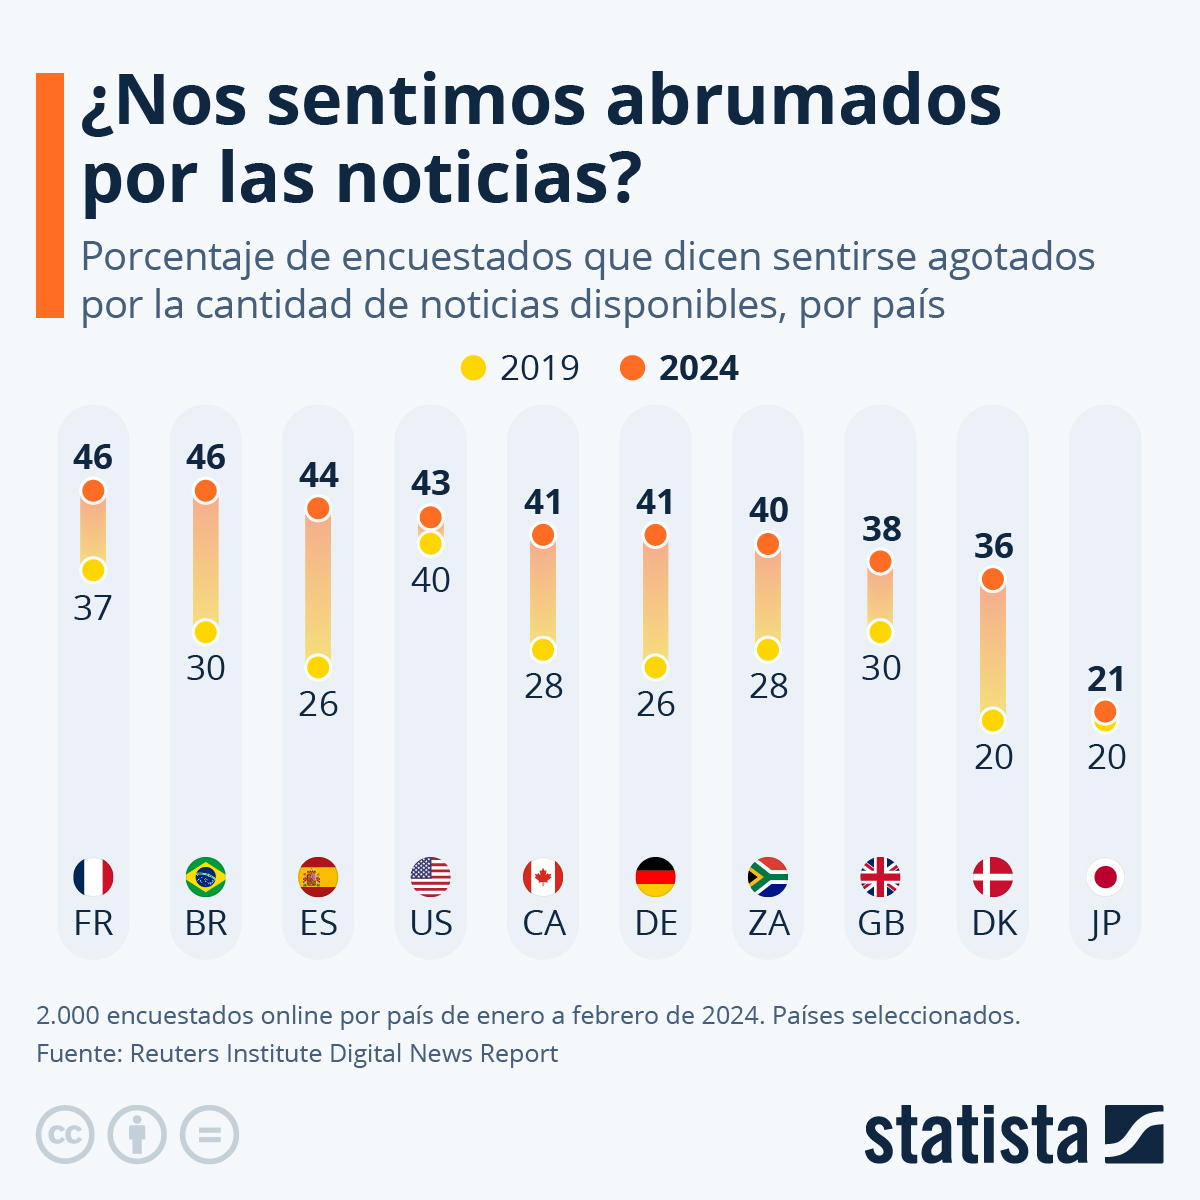
\includegraphics[width=0.7\textwidth]{graf3.jpeg}
    \caption{Gráfico sobre el porcentaje de personas que se sienten abrumadas por la cantidad de noticias.}
    \label{fig:graf3}
\end{figure}
\subsubsection{Análisis}

\paragraph{Proximidad:}
Las barras aparecen claramente \textbf{separadas por países}, lo que facilita percibirlas como \textbf{grupos diferenciados} y permite una \textbf{comparación más efectiva} entre ellos.

\paragraph{Semejanza:}
Se aprecia en la \textbf{diferenciación entre los años 2019 y 2024}, que comparten un mismo \textbf{estilo visual}, lo cual indica que poseen un \textbf{elemento en común}.

\paragraph{Figura - Fondo:}
Las barras \textbf{destacan con claridad sobre un fondo neutro y sencillo}, lo que facilita la \textbf{lectura} y evita \textbf{distracciones visuales}.

\paragraph{Conectividad:}
Los \textbf{puntos correspondientes a cada año} se encuentran \textbf{unidos mediante líneas}, lo cual ayuda a visualizar \textbf{tendencias de avance o retroceso} en los datos a lo largo del tiempo.

\paragraph{Simetría y orden:}
Las barras están ordenadas de izquierda a derecha según el \textbf{porcentaje de personas que se sienten más abrumadas} en 2024 hasta aquellas que se sienten menos abrumadas.

\subsubsection{Mejoras}

\paragraph{Cercamiento:}
Cada país aparece \textbf{enmarcado sobre un fondo gris}, aunque este resulta demasiado claro y apenas se distingue del fondo principal. Una \textbf{tonalidad ligeramente más opaca} permitiría reforzar el principio sin restar protagonismo a las barras.

\paragraph{Simetría y orden:}
Si bien el gráfico presenta un \textbf{orden interno}, la ausencia de un \textbf{criterio de organización más evidente} —por ejemplo, alfabético o geográfico— puede dificultar una interpretación inmediata. Una \textbf{reordenación más lógica de los países} mejoraría la comprensión sin necesidad de observar detenidamente el gráfico.

\end{document}
